% \subsubsection{Mô hình pre-trained }
% Một trong những thách thức lớn nhất của NLP là thiếu hụt dữ liệu huấn luyện. Mặc dù tổng thể có một lượng dữ liệu văn bản khổng lồ, nhưng để tạo ra các bộ dữ liệu cho các nhiệm vụ cụ thể, chúng ta cần phân chia chúng thành nhiều lĩnh vực rất đa dạng. Điều này dẫn đến việc chỉ có vài nghìn hoặc vài trăm nghìn mẫu huấn luyện được dán nhãn thủ công. Nếu muốn đạt được những cải tiến đáng kể, các mô hình NLP dựa trên học sâu đòi hỏi lượng dữ liệu lớn hơn nhiều - hàng triệu hoặc hàng tỷ mẫu huấn luyện được dán nhãn.

% Để giúp bù đắp khoảng trống về dữ liệu này, các nhà nghiên cứu đã phát triển các kỹ thuật khác nhau để huấn luyện sử dụng khối lượng văn bản khổng lồ không dán nhãn trên web (được gọi là pre-training). Các mô hình này được tiền huấn luyện này sau đó có thể được tinh chỉnh (fine-tuned) trên các bộ dữ liệu nhỏ hơn cho các nhiệm vụ cụ thể, chẳng hạn như giải quyết các vấn đề như trả lời câu hỏi, phân tích cảm xúc. Cách tiếp cận này đã mang lại những cải thiện đáng kể so với việc huấn luyện từ đầu trên các bộ dữ liệu nhỏ hơn cho các nhiệm vụ cụ thể. 

% https://arxiv.org/abs/1810.04805
\subsubsection{Giới thiệu BERT}
Vào cuối năm 2018, các nhà nghiên cứu tại Google AI Language đã công bố một kỹ thuật mới được gọi là BERT ({\bf B}idirectional {\bf E}ncoder {\bf R}epresentations from {\bf T}ransformers) - một bước đột phá lớn đã gây tiếng vang trong cộng đồng Học sâu bởi hiệu suất đáng kinh ngạc của nó. Trong bài báo BERT: Pre-training of Deep Bidirectional Transformers for Language Understanding\cite{bert} các tác giả đã nêu ra những cải tiến của model BERT trong các tác vụ\cite{webpage20}:

\begin{itemize}
    \item Tăng GLUE score (General Language Understanding Evaluation score), một chỉ số tổng quát đánh giá mức độ hiểu ngôn ngữ lên 80.5\%.
    \item Tăng accuracy trên bộ dữ liệu MultiNLI đánh giá tác vụ quan hệ văn bản (text entailment) lên 86.7\%.
    \item Tăng accuracy F1 score trên bộ dữ liệu SQuAD v1.1 đánh giá tác vụ question and answering lên 93.2\%.
\end{itemize}
% https://medium.com/@samia.khalid/bert-explained-a-complete-guide-with-theory-and-tutorial-3ac9ebc8fa7c
Về cơ bản, nhiệm vụ mà các mô hình ngôn ngữ cố gắng giải quyết là  ``điền vào chỗ trống'' dựa trên ngữ cảnh. Ví dụ, với câu: ``Tôi đi chợ và mua một \_\_\_\_ giày.''
Một mô hình ngôn ngữ có thể hoàn thành câu bằng cách dự đoán từ điền vào chỗ trống\cite{webpage19}:

\begin{itemize}
    \item ``đôi'' với tỉ lệ 80\% vì ``đôi'' là cách đếm thông dụng cho giày.
    \item ``chiếc'' với tỉ lệ 20\% vì đôi khi người ta cũng một chiếc giày.
\end{itemize}

Trước khi BERT được công bố, những mô hình ngôn ngữ sẽ xem xét chuỗi văn bản này trong quá trình huấn luyện theo hướng từ trái sang phải hoặc kết hợp cả hai hướng. Cách tiếp cận đơn hướng này hoạt động tốt cho việc tạo câu, chúng ta có thể dự đoán từ tiếp theo, thêm nó vào chuỗi, sau đó dự đoán từ tiếp theo sau đó cho đến khi có một câu hoàn chỉnh.

Tuy nhiên, với sự xuất hiện của BERT, mô hình ngôn ngữ giờ đây được huấn luyện theo hai hướng, đã làm thay đổi cách tiếp cận ngữ cảnh của từ. Điều này có nghĩa là bây giờ chúng ta có thể có được hiểu biết sâu sắc hơn về bối cảnh so với các mô hình ngôn ngữ một hướng.

\begin{figure}[htb]
    \centering
    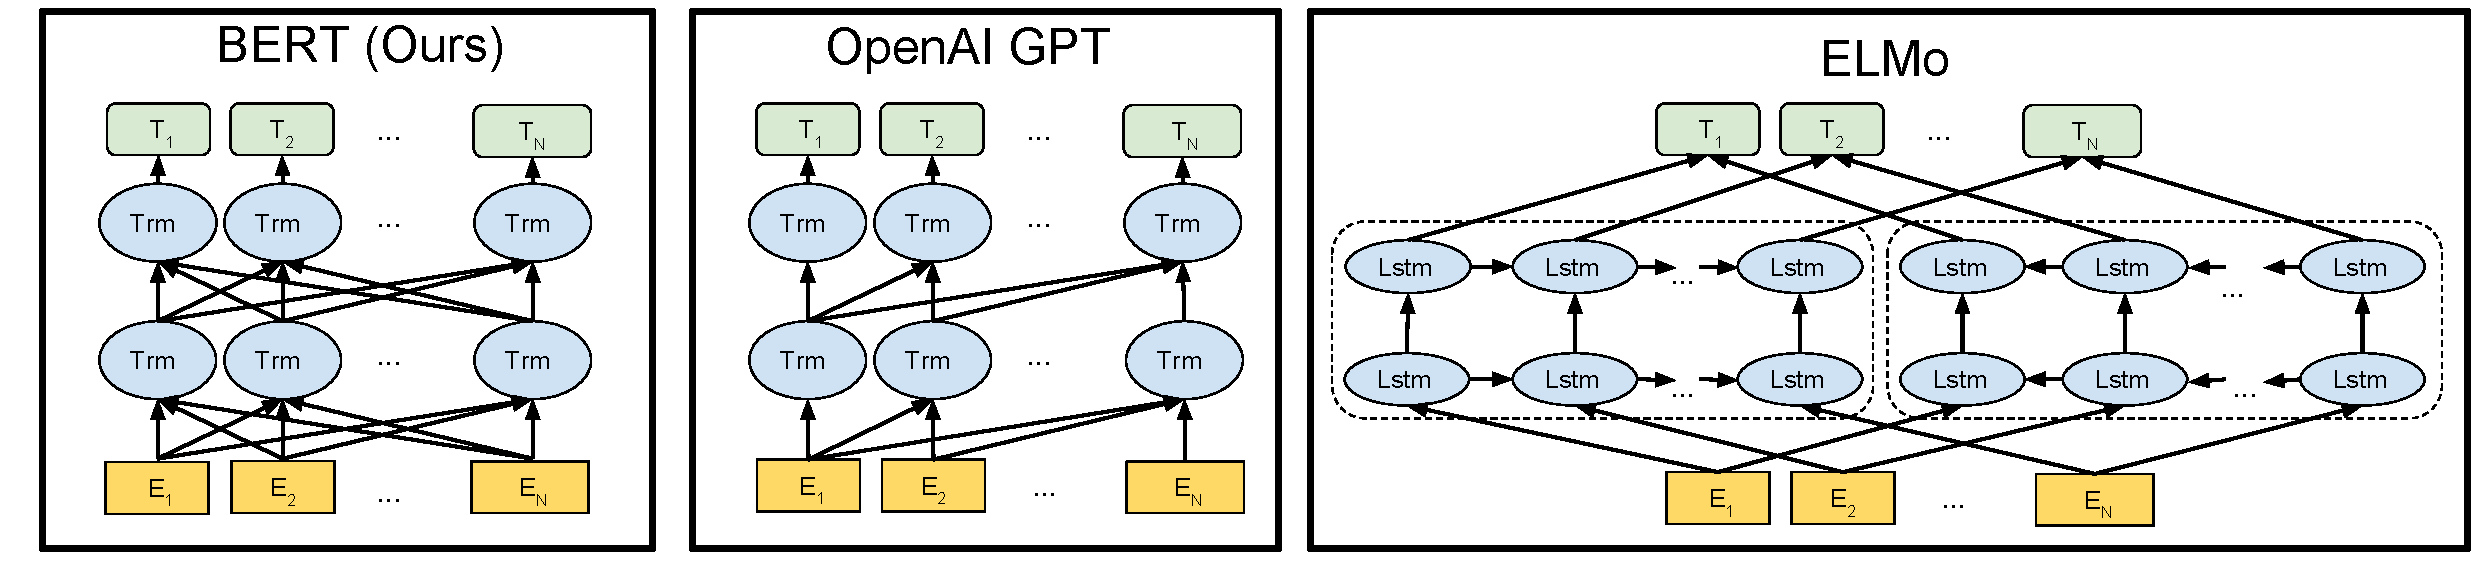
\includegraphics[width=\textwidth]{image/BERT_comparisons.pdf}
    \caption[Sự khác nhau giữa các kiến trúc mô hình pre-trained]{Sự khác nhau giữa các kiến trúc mô hình pre-trained. BERT sử dụng bidirectional Transformer. OpenAI GPT sử dụng Transformer theo hướng trái sang phải. ELMo sử dụng kết hợp đầu ra của hai LSTM được huấn luyện độc lập theo hướng trái sang phải và phải sang trái. Trong ba mô hình này, chỉ có BERT học được biểu diễn của từ ngữ phụ thuộc lẫn nhau vào cả ngữ cảnh trước và sau ở tất cả các layer. \cite{bert}}
    \label{figure:BERT_comparisons}
\end{figure}

Thay vì dự đoán từ tiếp theo trong chuỗi, BERT sử dụng một kỹ thuật mới gọi là Masked LM (MLM). Kỹ thuật này hoạt động bằng cách ngẫu nhiên che khuất một số từ trong câu và sau đó BERT cố gắng dự đoán các từ đó. Che khuất ở đây có nghĩa là mô hình sẽ xem xét cả hai hướng của câu, sử dụng toàn bộ ngữ cảnh của câu, bao gồm cả các từ trước và sau từ bị che khuất, để dự đoán từ đó. Không giống như các mô hình ngôn ngữ trước đây, BERT có thể tính đến cả token trước và token sau cùng một lúc. Các mô hình LSTM kết hợp trái-sang-phải và phải-sang-trái hiện nay không thể làm được điều này mặc dù trên thực tế, chính xác hơn chúng ta có thể nói rằng đó là huấn luyện không hướng (non-directional).

\subsubsection{Pre-training BERT}

BERT được huấn luyện dựa trên Transformer, mục tiêu là tạo mô hình biểu diễn ngôn ngữ, vì vậy BERT chỉ cần phần Encoder. Đầu vào cho bộ mã hóa của BERT là một chuỗi các token, được chuyển đổi thành các vector và sau đó được xử lý trong mạng nơ-ron. Tuy nhiên, trước khi quá trình xử lý bắt đầu, BERT cần một số dữ liệu bổ sung vào input được trình bày trong hình \ref{figure:Input_Emebeddings}:

\begin{itemize}
    \item \textbf{Nhúng từ (token embedding)}: Ký hiệu {\tt [CLS]} được thêm vào các token từ đầu vào ở đầu câu đầu tiên và ký hiệu {\tt [SEP]} được chèn vào cuối mỗi câu.
    \item \textbf{Nhúng câu (segment embedding)}: Thêm một ký hiệu chỉ thị Câu A hoặc Câu B cho mỗi token. Điều này cho phép bộ mã hóa phân biệt giữa các câu.
    \item \textbf{Nhúng vị trí (position embedding)}: Thêm một vector nhúng vị trí cho mỗi token trong chuỗi. Điều này cho phép mô hình biết vị trí của mỗi token trong chuỗi.
\end{itemize}

\begin{figure}[htb]
    \centering
    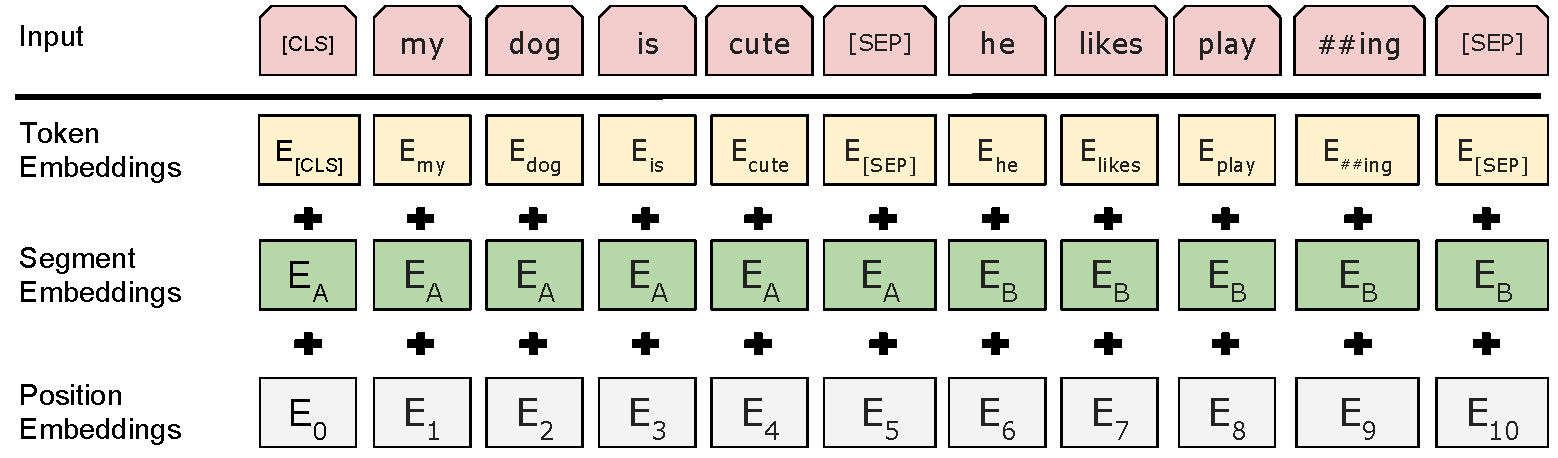
\includegraphics[width=\textwidth]{image/Input_Emebeddings.pdf}
    \caption{Biểu diễn đầu vào của BERT: Bao gồm các token embedding, token segment và token position.\cite{bert}}
    \label{figure:Input_Emebeddings}
\end{figure}

Về bản chất, Transformer sẽ ánh xạ chuỗi ký tự đầu vào thành chuỗi ký tự đầu ra, do đó đầu ra cũng là một chuỗi các vector tương ứng giữa các token đầu vào và đầu ra ở cùng chỉ số. Như đã đề cập trước đó, BERT sẽ không dự đoán từ tiếp theo trong câu. Quá trình huấn luyện sử dụng hai chiến lược sau\cite{webpage20}:
% https://phamdinhkhanh.github.io/2020/05/23/BERTModel.html#23-masked-ml-mlm
\begin{enumerate}
    \item \textbf{Masked Language Modeling (MLM):}
          Masked LM là một tác vụ cho phép chúng ta fine-tuning lại các biểu diễn từ trên các bộ dữ liệu unsupervised-text bất kỳ. Chúng ta có thể áp dụng Masked LM cho những ngôn ngữ khác nhau để tạo ra biểu diễn embedding cho chúng. Các bộ dữ liệu của tiếng anh có kích thước lên tới vài vài trăm tới vài nghìn GB được huấn luyện trên BERT đã tạo ra những kết quả khá ấn tượng.

          Theo đó:
          \begin{itemize}
              \item Khoảng 15\% các token của câu input được thay thế bởi token {\tt [MASK]} trước khi truyền vào model đại diện cho những từ bị che dấu (masked). Mô hình sẽ dựa trên các từ không được che (non-masked) dấu xung quanh và đồng thời là bối cảnh của {\tt [MASK]} để dự báo giá trị gốc của từ được che dấu. Số lượng từ được che dấu được lựa chọn là một số ít (15\%) để tỷ lệ bối cảnh chiếm nhiều hơn (85\%).
              \item Bản chất của kiến trúc BERT vẫn là một mô hình seq2seq gồm 2 phase encoder giúp embedding các từ input và decoder giúp tìm ra phân phối xác suất của các từ ở output. Kiến trúc Transfomer encoder được giữ lại trong tác vụ Masked LM. Sau khi thực hiện self-attention và feed forward ta sẽ thu được các vector embedding ở output là $O_1, O_2,…, O_n$
              \item Để tính toán phân phối xác suất cho từ output, chúng ta thêm một Fully connect layer ngay sau Transformer Encoder. Hàm softmax có tác dụng tính toán phân phối xác suất. Số lượng units của fully connected layer phải bằng với kích thước của từ điển.
              \item Cuối cùng ta thu được vector nhúng của mỗi một từ tại vị trí {\tt [MASK]} sẽ là embedding vector giảm chiều của vector $O_i$ sau khi đi qua fully connected layer.
          \end{itemize}

          Hàm loss function của BERT sẽ bỏ qua mất mát của những từ không bị che và chỉ nhận của những từ bị che dấu. Do đó mô hình sẽ hội tụ lâu hơn nhưng đây là đặc tính bù trừ cho sự gia tăng ý thức về bối cảnh. Việc lựa chọn ngẫu nhiên 15\% số lượng các từ bị che dấu cũng tạo ra vô số các kịch bản input cho mô hình huấn luyện nên mô hình sẽ cần phải huấn luyện rất lâu mới học được toàn diện các khả năng.
    \item \textbf{Next Sentence Prediction (NSP):}

          Đây là một bài toán phân loại học có giám sát với 2 nhãn (hay còn gọi là phân loại nhị phân). Input đầu vào của mô hình là một cặp câu (pair-sequence) sao cho 50\% câu thứ 2 được lựa chọn là câu tiếp theo của câu thứ nhất và 50\% được lựa chọn một cách ngẫu nhiên từ bộ văn bản mà không có mối liên hệ gì với câu thứ nhất. Nhãn của mô hình sẽ tương ứng với {\tt {\small IsNext}} khi cặp câu là liên tiếp hoặc {\tt {\small NotNext}} nếu cặp câu không liên tiếp.

          Cũng tương tự như trên, chúng ta cần đánh dấu các vị trí đầu câu thứ nhất bằng token {\tt [CLS]} và vị trí cuối các câu bằng token {\tt [SEP]}. Các token này có tác dụng nhận biết các vị trí bắt đầu và kết thúc của từng câu thứ nhất và thứ hai.

          Mô hình sẽ dựa vào các vector embedding của token {\tt [CLS]} để dự đoán xem cặp câu đó có phải là liên tiếp hay không. Để dự đoán, chúng ta sẽ thêm một fully connected layer với 2 units (tương ứng với 2 nhãn) ngay sau vector embedding của token {\tt [CLS]}. Hàm softmax sẽ giúp tính toán phân phối xác suất của 2 nhãn. Cuối cùng, mô hình sẽ dự đoán nhãn có xác suất cao nhất là nhãn cuối cùng của cặp câu.
\end{enumerate}

\subsubsection{Tinh chỉnh \textit(fine-tuning) BERT}

BERT đã vượt trội so với các phương pháp tối ưu (state-of-the-art) trước đây trên nhiều tác vụ khác nhau trong lĩnh vực hiểu ngôn ngữ tổng quát, chẳng hạn như suy luận ngôn ngữ tự nhiên, phân tích tình cảm và trả lời câu hỏi.
Nếu muốn tinh chỉnh BERT cho một nhiệm vụ cụ thể dựa trên tập dữ liệu, việc cần làm là thêm một layer phía sau phần Encoder của BERT như hình \ref{figure:BERT_fine_tuning}.

\begin{figure}[htb]
    \centering
    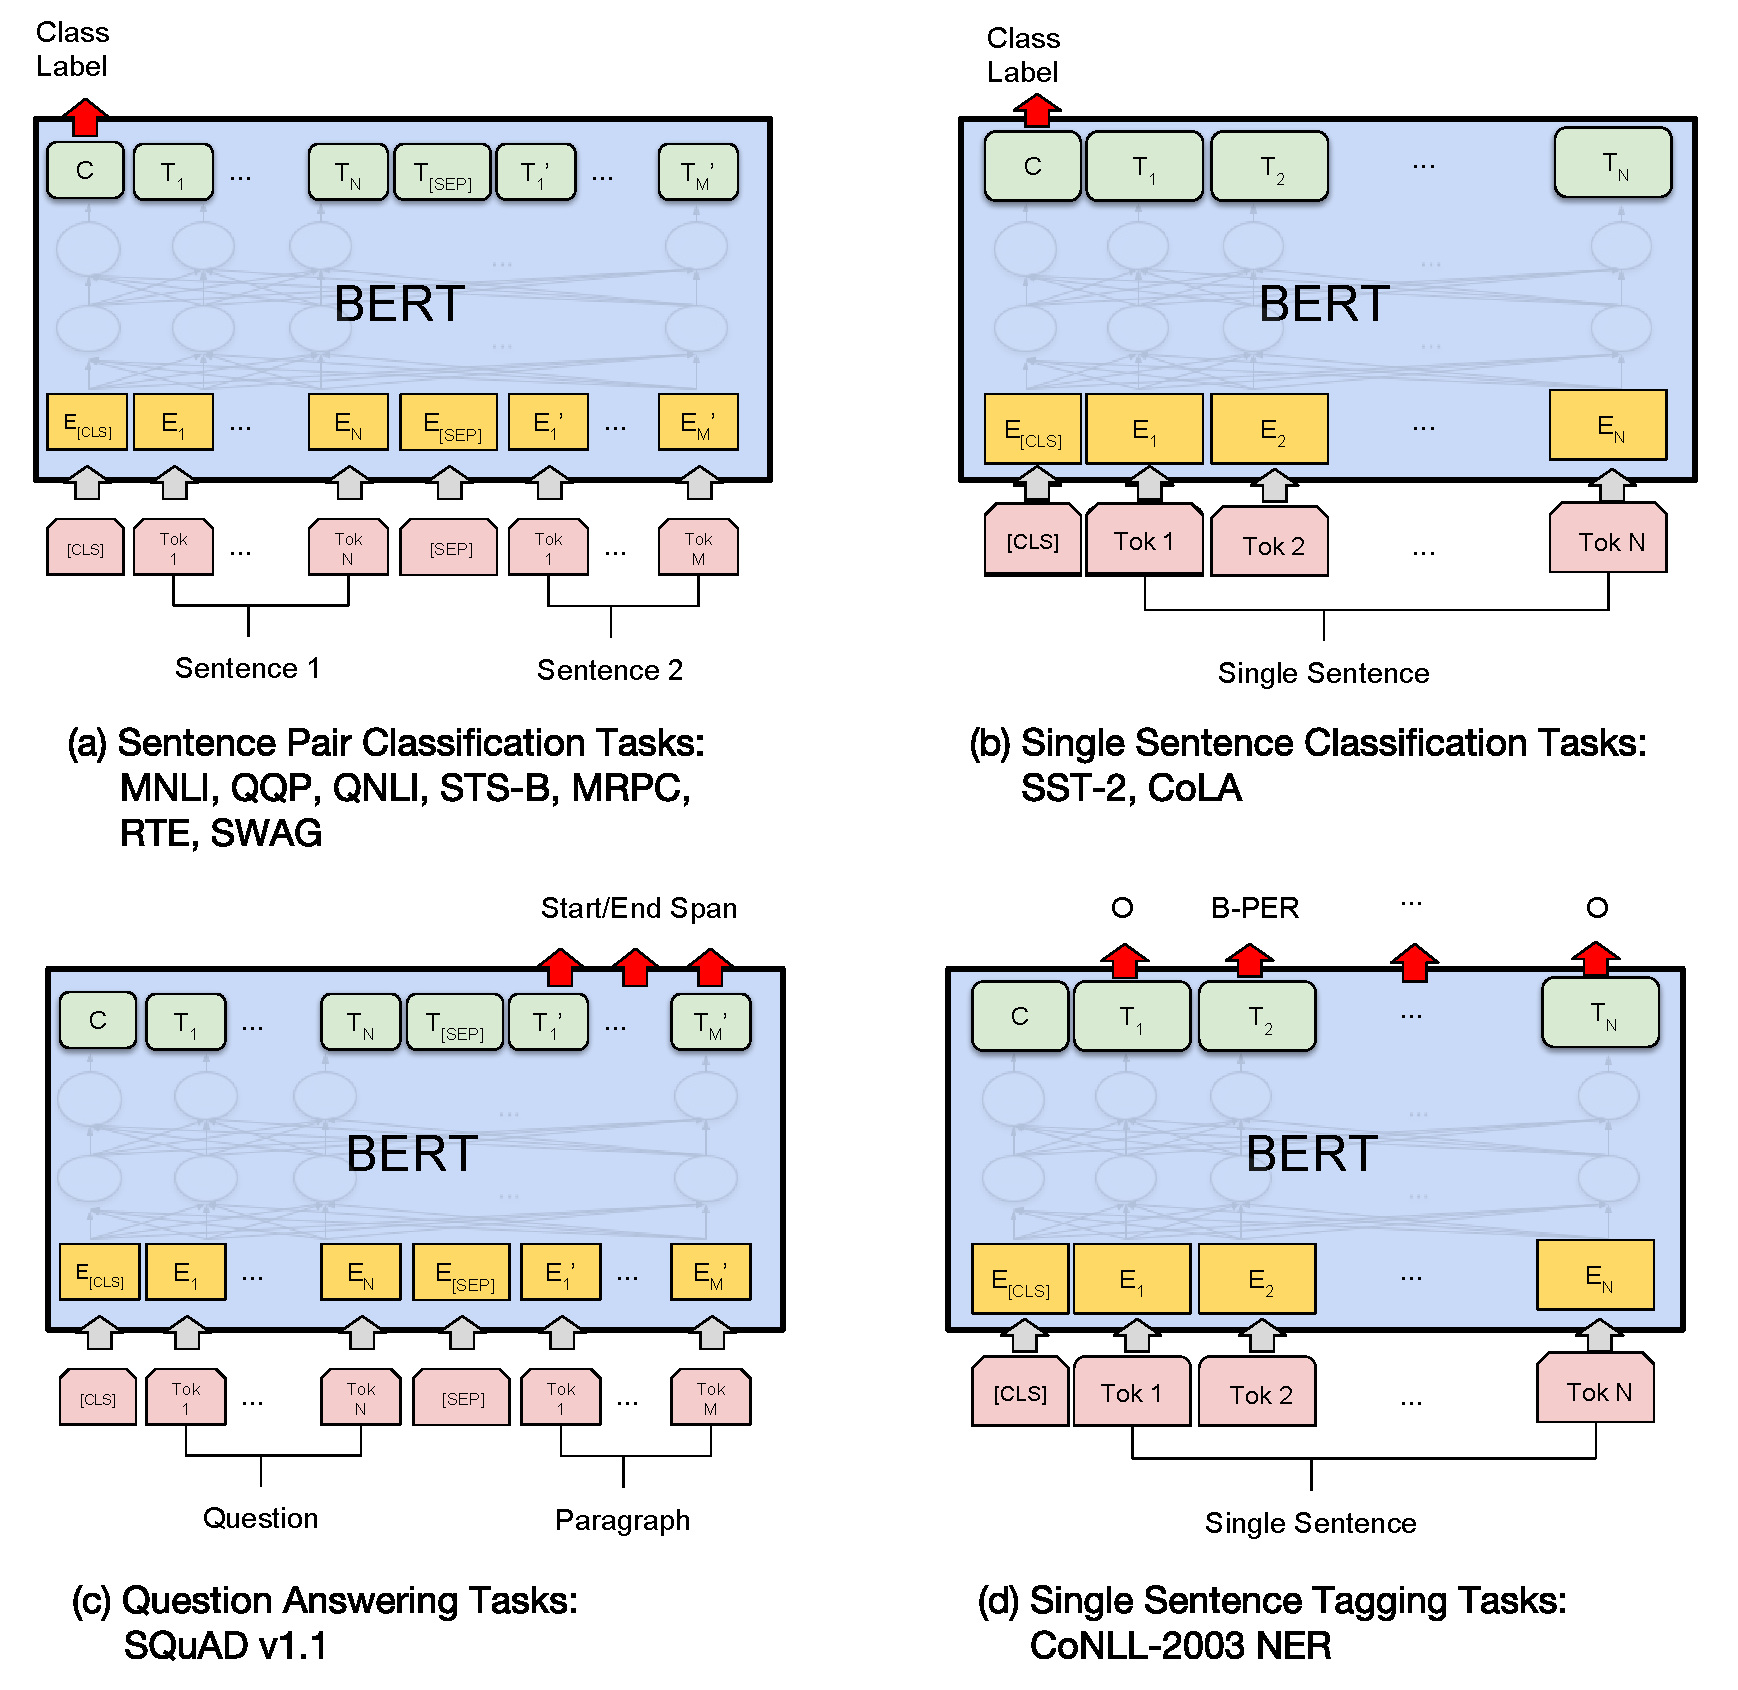
\includegraphics[width=\textwidth]{image/BERT_fine_tune.pdf}
    \caption{Minh họa việc tinh chỉnh BERT cho các tác vụ khác nhau \cite{bert}}
    \label{figure:BERT_fine_tuning}
\end{figure}

Ví dụ, giả sử chúng ta đang tạo một ứng dụng trả lời câu hỏi (question answering). Về bản chất, đây là một tác vụ dự đoán - khi nhận được một câu hỏi làm đầu vào, mục tiêu của ứng dụng là xác định câu trả lời đúng có trong một ngữ liệu nào đó. Vì vậy, với một câu hỏi và một đoạn ngữ cảnh, mô hình sẽ dự đoán một token bắt đầu và một token kết thúc trong đoạn văn đó, đoạn văn được lấy từ 2 token này có khả năng là trả lời chính xác.

Ví dụ:

\begin{itemize}
    \item Input Question:
            % sự kết tủa của giọt nước khi va chạm với những tỉnh thể băng xảy ra ở đâu để tạo thành tuyết?
            {\raggedright\texttt{Where do water droplets collide with ice crystals to form precipitation?}\par}

    \item Input Paragraph:
            % sự kết tủa của giọt nước để trở thành tuyết xảy ra khi va chạm với những hạt mưa hoặc tỉnh thể băng ở bên trong đám mây.
            {\raggedright\texttt{[\dots] Precipitation forms as smaller droplets coalesce via collision with other rain drops or ice crystals within a cloud. [\dots]}\par}

    \item Output Answer:
            % ở bên trong đám mây
            \texttt{within a cloud}
\end{itemize}

Tương tự như các tác vụ liên quan đến cặp câu được đề cập ở phần dự đoán câu tiếp theo, ở phần này câu hỏi sẽ trở thành câu đầu tiên và đoạn văn là câu thứ hai trong chuỗi đầu vào. Tuy nhiên, lần này có thêm hai tham số mới được học trong quá trình tinh chỉnh: một vector bắt đầu và một vector kết thúc.

% https://phamdinhkhanh.github.io/2020/05/23/BERTModel.html#3-c%C3%A1c-ki%E1%BA%BFn-tr%C3%BAc-model-bert
\subsubsection{Những kiến trúc của BERT}
Hiện tại có nhiều phiên bản khác nhau của model BERT. Các phiên bản đều dựa trên việc thay đổi kiến trúc của Transformer tập trung ở 3 tham số: $L$: số lượng các block sub-layers trong transformer, $H$: kích thước của embedding vector (hay còn gọi là hidden size), $A$: Số lượng head trong multi-head layer, mỗi một head sẽ thực hiện một self-attention. Tên gọi của 2 kiến trúc bao gồm:
\begin{itemize}
    \item $BERT_{BASE}$ ($L$=12, $H$=768, $A$=12): Tổng tham số 110 triệu.
    \item $BERT_{LARGE}$ ($L$=24, $H$=1024, $A$=16): Tổng tham số 340 triệu.
\end{itemize}
Như vậy ở kiến trúc BERT Large chúng ta tăng gấp đôi số layer, tăng kích thước hidden size của embedding vector gấp 1.33 lần và tăng số lượng head trong multi-head layer gấp 1.33 lần.

% https://viblo.asia/p/bert-roberta-phobert-bertweet-ung-dung-state-of-the-art-pre-trained-model-cho-bai-toan-phan-loai-van-ban-4P856PEWZY3
\subsubsection{PhoBERT}

PhoBERT là mô hình ngôn ngữ tiền huấn luyện (pre-trained language model) đầu tiên được phát triển dành riêng cho tiếng Việt. Mô hình do VinAI giới thiệu vào năm 2020 này được xây dựng dựa trên kiến trúc RoBERTa\footnote{\url{https://doi.org/10.48550/arXiv.1907.11692}} của Facebook, một phiên bản cải tiến so với BERT, và được huấn luyện trên một tập dữ liệu khổng lồ gồm văn bản tiếng Việt\cite{webpage21}.

Những đặc điểm chính của PhoBERT bao gồm:
\begin{itemize}
    \item Tiền huấn luyện đơn ngôn ngữ (Monolingual language model): PhoBERT chỉ được huấn luyện trên dữ liệu tiếng Việt, giúp mô hình hiểu và xử lý ngôn ngữ tiếng Việt một cách hiệu quả hơn.
    \item Kiến trúc RoBERTa: PhoBERT sử dụng kiến trúc RoBERTa, một phiên bản cải tiến của BERT, giúp mô hình đạt được hiệu suất tốt hơn trong nhiều nhiệm vụ xử lý ngôn ngữ tự nhiên (NLP).
    \item Tập dữ liệu khổng lồ: PhoBERT được huấn luyện trên một tập dữ liệu khổng lồ gồm văn bản tiếng Việt, bao gồm khoảng 1GB dữ liệu Wikipedia tiếng Việt và 20GB nguồn tin tức tiếng Việt.
    \item Bộ chia tách từ RDRSegmenter: PhoBERT sử dụng bộ chia tách từ RDRSegmenter của VnCoreNLP\footnote{\url{https://github.com/vncorenlp/VnCoreNLP}} để tách từ cho dữ liệu đầu vào trước khi đưa vào mô hình.
    \item Nhiệm vụ huấn luyện: Vì tiếp cận theo kiến trúc RoBERTa, PhoBERT chỉ sử dụng nhiệm vụ Masked Language Model (MLM) để huấn luyện, giúp mô hình học cách dự đoán từ thiếu trong một câu dựa vào các từ ngữ cảnh.
\end{itemize}

PhoBERT được giới thiệu với 2 phiên bản, tương tự như BERT:
\begin{itemize}
    \item $PhoBERT_{BASE}$: Có 12 khối transformer.
    \item $PhoBERT_{LARGE}$: Có 24 khối transformer.
\end{itemize}


